\documentclass[tikz,border=2pt]{standalone}
\usepackage{graphicx}
\usepackage{tikz}
\usetikzlibrary{arrows.meta}
\begin{document}
\begin{tikzpicture}
  \node[anchor=south west, inner sep=0] (img) at (0,0) {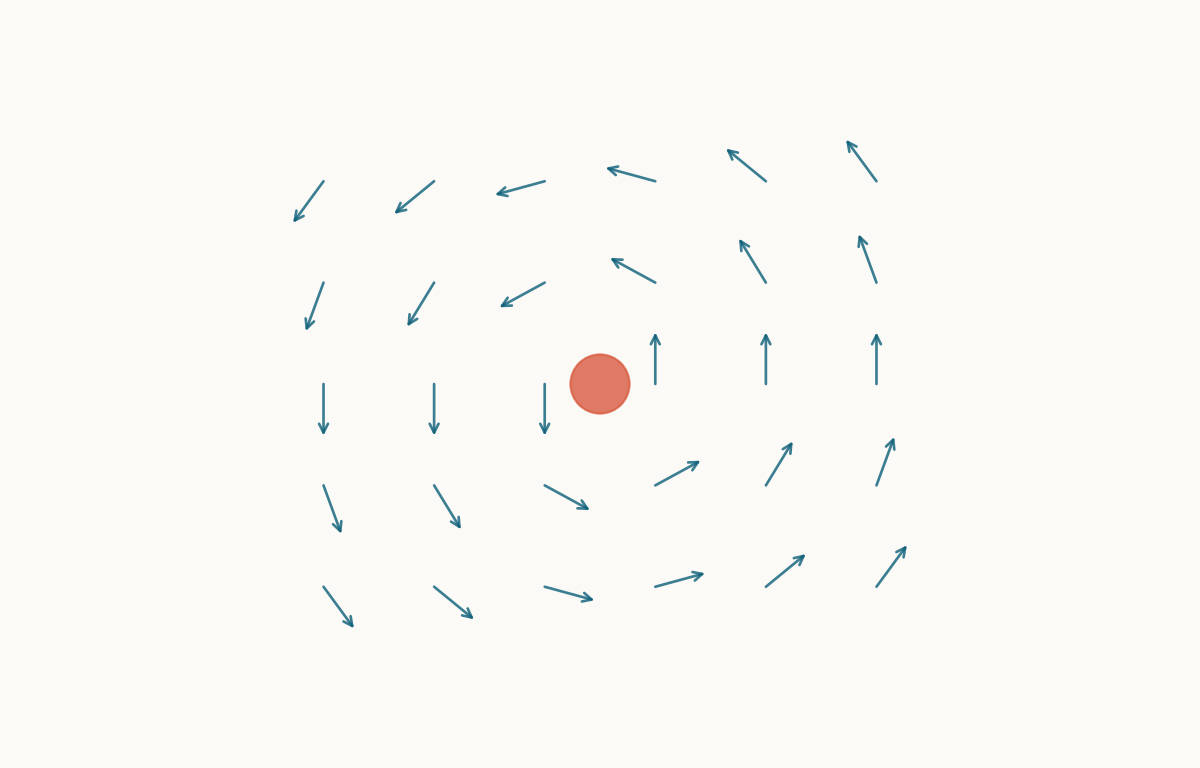
\includegraphics[width=12cm]{ch017maxwelltheoryfrompotentials-01-potential-field.png}};
  \begin{scope}[
    x={(img.south east)},
    y={(img.north west)},
    labelbox/.style={font=\sffamily\small, fill=white, fill opacity=0.88, text opacity=1, rounded corners=1.5pt, inner xsep=3pt, inner ysep=2pt, draw=black!20},
    callout/.style={-{Latex[length=2.2mm]}, line width=0.7pt, black!70},
  ]
    \node[labelbox, anchor=north west] at (0.035,0.965) {potentials producing fields};
    \draw[callout] (0.16,0.18) -- (0.33,0.18) node[midway, above, labelbox] {potential contours};
    \draw[callout] (0.74,0.78) -- (0.55,0.58) node[pos=0, above, labelbox] {field arrows};
    \node[labelbox, anchor=south east] at (0.965,0.055) {derivative};
  \end{scope}
\end{tikzpicture}
\end{document}
